\section{Auswertung}
\label{sec:Auswertung}

\subsection{Gegengekoppelter Verstärker}

Die Werte der vier verschiedenen Widerstandskombinationen sind in den Tabellen \ref{tab:gegen_kombi_1}, \ref{tab:gegen_kombi_2}, \ref{tab:gegen_kombi_3} und \ref{tab:gegen_kombi_4} eingetragen.
Die Fehler werden wie folgt angenommen: $\sigma_\nu = \num{0.1} \nu, \sigma_U = \SI{10}{\milli\volt}$. Graphisch dargestellt sind die Messwerte sowie ein Fit an die Messwerte, die händisch der Flanke zugeordnet werden, in Abbildung \ref{fig:gegen} zu sehen.
\begin{figure}
  \centering
  \includegraphics[width=1.2\textwidth]{build/gegen.pdf}
  \caption{Messwerte und Flankenfit aller vier Widerstandskombinationen mit $V'_\text{Theorie} = R_N / R_1$.}
  \label{fig:gegen}
\end{figure}
Dieser Fit folgt der Gleichung:
\begin{align}
  \ln(V') = m \ln(\nu/\si{\kilo\hertz}) + b.
\end{align}
Dabei ergeben sich die Werte aus Tabelle \ref{tab:gegen_ergebnisse}. Dort ist auch die Grenzfrequenz eingetragen, die aus dem Schnittpunkt der gefitteten Graden mit der Linie auf Höhe von $V'_\text{Theorie}/\sqrt{2}$ beziehungsweise $V'_\text{Theorie}\cdot\sqrt{2}$ gewonnen wird. Außerdem ist in Tabelle \ref{tab:gegen_ergebnisse} der Mittelwert der Messwerte der Plateaus angegeben, sowie die prozentuale Abweichung von $V'_\text{Theorie}$.

\begin{table}[h]
  \centering
  \begin{tabular}{S[table-format=1.0]
    S[table-format=2.3] @{${}\pm{}$} S[table-format=1.3]
    S[table-format=2.2] @{${}\pm{}$} S[table-format=1.2]
    S[table-format=3.0]
    S[table-format=1.4] @{${}\pm{}$} S[table-format=1.4]
    S[table-format=1.0] @{${}\pm{}$} S[table-format=1.0]}
    \toprule
    {i} & \multicolumn{2}{c}{$m$} & \multicolumn{2}{c}{$b$} & {$\nu'_\text{g}\:/\:\si{\kilo\hertz}$} & \multicolumn{2}{c}{$\bar V'_\text{Plateau}$} &
    \multicolumn{2}{c}{$\Delta_{V'}\:/\:\si{\percent}$}\\
    \midrule
    1 & -0.832 & 0.007 & 4.49 & 0.05 & 335 & 1.01 & 0.02 & 1 & 3\\
    2 & 0.16 & 0.07 & -2.9 & 0.5 & 368 & 0.1038 & 0.0004 & 3 & 5\\
    3 & -0.5 & 0.1 & 3.1 & 0.7 & 154 & 2.00 & 0.02 & 6 & 5\\
    4 & -0.87 & 0.04 & 4.7 & 0.2 & 25 & 9.6 & 0.2 & 3 & 5\\
    \bottomrule
  \end{tabular}
  \caption{Ergebnisse aus der Messung mit gegengeschaltetem Operationsverstärker. Dabei ist $i$ die Nummer der Widerstandskombination; definiert in den Tabellen der Messwerte im Anhang.}
  \label{tab:gegen_ergebnisse}
\end{table}

Nun wird die Beziehung $\nu'_\text{g} V'=$ const überprüft. Es ergeben sich die Werte:
\begin{align*}
  \nu'_{\text{g}, 1} V'_1 = \SI{335(2)}{\kilo\hertz} \quad \nu'_{\text{g}, 2} V'_2 = \SI{37(2)}{\kilo\hertz}\\ \nu'_{\text{g}, 3} V'_3 = \SI{328(17)}{\kilo\hertz} \quad \nu'_{\text{g}, 4} V'_4 = \SI{245(12)}{\kilo\hertz},
\end{align*}
wobei der Index die jeweilige Widerstandskombination angibt. Da die zweite Kombination sich stark von den anderen unterscheidet, dadurch dass sie abschwächt und nicht verstärkt, wird sie zur Überprüfung der Konstanz nicht herangezogen.
Der Mittelwert aus den anderen Kombinationen beträgt:
\begin{align*}
  \frac{1}{3}\sum_{i=1, i\neq2}^4 \nu'_{\text{g}, \text{i}} V'_\text{i} = \SI{303(40)}{\kilo\hertz}.
\end{align*}

Außerdem wird für den gegengekoppelten Verstärker die endliche Leerlaufverstärkung $V$ mit Formel \eqref{eqn:leerlaufverst} abgeschätzt. Die vier einzelnen Werte sind:
\begin{align*}
  V_1 = \num{-70(10)} \quad V_2 = \num{-3(5)} \quad V_3 = \num{32(26)} \quad V_4 = \num{300(500)}.
\end{align*}

Zuletzt wird in Abbildung \ref{fig:phase} die Abhängigkeit der Phasendifferenz zwischen Eingangs- und Ausgangsspannung von der Frequenz dargestellt.

\begin{figure}
  \centering
  \includegraphics[width=0.8\textwidth]{build/phasen.pdf}
  \caption{Messwerte der Phasendifferenz zwischen Eingangs- und Ausgangsspannung aller vier Widerstandskombinationen.}
  \label{fig:phase}
\end{figure}

\subsection{Umkehr-Integrator}

Zunächst werden auf die Schaltung des Umkehr-Integrators drei verschiedene Eingangsspannung gegeben.
In der Schaltung werden für Widerstand und Kondensator Bauteile mit folgenden  Werten verwendet:
\begin{align*}
  R = \SI{99.7(5)}{\kilo\ohm} \quad C = \SI{970(10)}{\nano\farad}.
\end{align*}
Der Verlauf der Ausgangsspannung sowie der Eingangsspannung sind in den Abbildungen \ref{fig:int_recht}, \ref{fig:int_drei} und \ref{fig:int_sin} zu sehen. Dabei ist die Eingangsspannung in orange und die Ausgangsspannung in grün abgebildet.

\begin{figure}
  \centering
  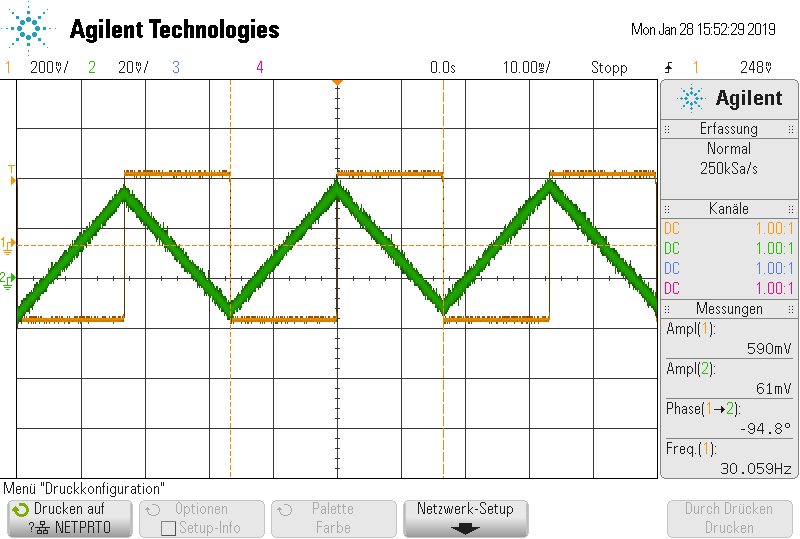
\includegraphics[width=0.8\textwidth]{Schlager/scope_16.png}
  \caption{Das Oszilloskopbild des Umkehr-Integrators bei angelegter Rechteckspannung.}
  \label{fig:int_recht}
\end{figure}
\begin{figure}
  \centering
  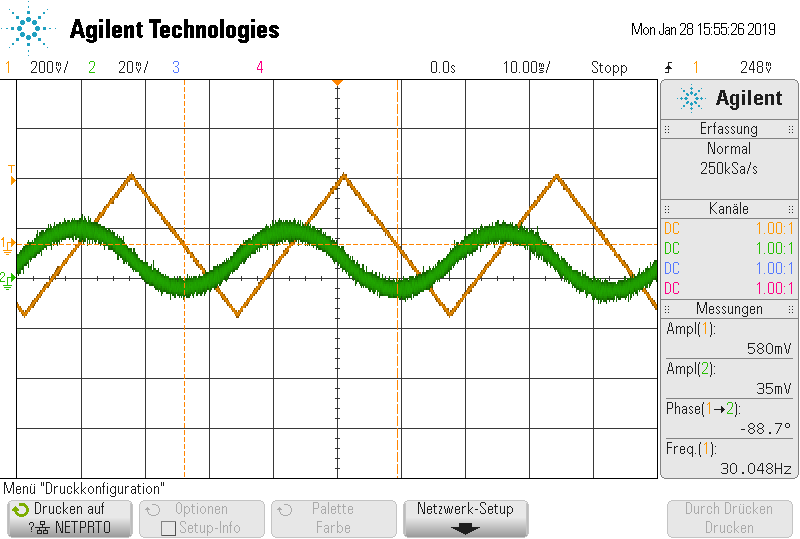
\includegraphics[width=0.8\textwidth]{Schlager/scope_17.png}
  \caption{Das Oszilloskopbild des Umkehr-Integrators bei angelegter Dreiecksspannung.}
  \label{fig:int_drei}
\end{figure}
\begin{figure}
  \centering
  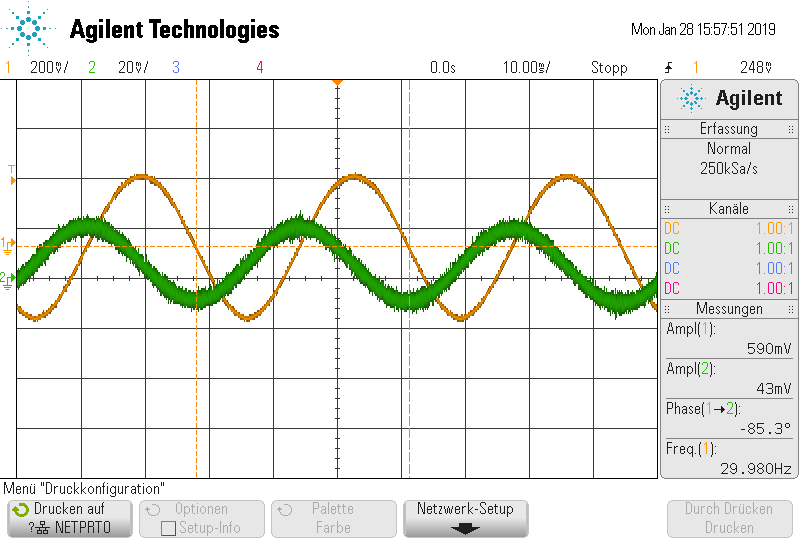
\includegraphics[width=0.8\textwidth]{Schlager/scope_18.png}
  \caption{Das Oszilloskopbild des Umkehr-Integrators bei angelegter Sinusspannung.}
  \label{fig:int_sin}
\end{figure}

Außerdem wird die Verstärkung $V' = U_\text{A}/U_0$ gegen die Kreisfrequenz $\omega$ aufgetragen. Dabei ist die Eingangsspannung sinusförmig. Die Messwerte sind in Tabelle \ref{tab:int_werte} zu finden.
Die Fitfunktion nach Formel \eqref{eqn:int_aus} lautet:
\begin{align}
  V' = \frac{1}{k \omega}.
\end{align}
Aus dem Fit, der zusammen mit den Messwerten in Abbildung \ref{fig:int_fit} zu sehen ist, folgt:
\begin{align*}
  k = \SI{0.062(3)}{\ohm\farad}.
\intertext{Die prozentuale Abweichung von dem nach Formel \eqref{eqn:int_aus} erwarteten Wert beträgt:}
  \Delta_{k, RC} = \SI{36(3)}{\percent}.
\end{align*}

\begin{figure}
  \centering
  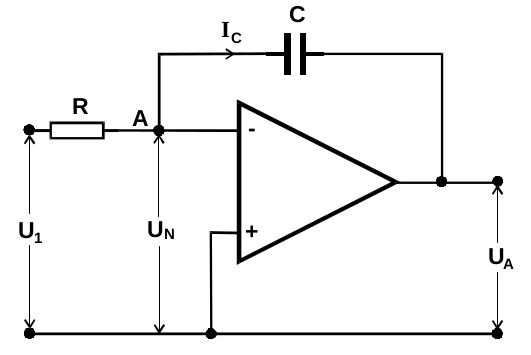
\includegraphics[width=0.8\textwidth]{build/integrator.pdf}
  \caption{Die frequenzabhängige Verstärkung des Umkehr-Integrators bei angelegter Sinusspannung.}
  \label{fig:int_fit}
\end{figure}

\subsection{Umkehr-Differentiator}

Zunächst werden auf die Schaltung des Umkehr-Differentiators drei verschiedene Eingangsspannung gegeben.
In der Schaltung werden für Widerstand und Kondensator Bauteile mit folgenden  Werten verwendet:
\begin{align*}
  R = \SI{1.002(50)}{\kilo\ohm} \quad C = \SI{970(10)}{\nano\farad}.
\end{align*}
Der Verlauf der Ausgangsspannung sowie der Eingangsspannung sind in den Abbildungen \ref{fig:diff_recht}, \ref{fig:diff_drei} und \ref{fig:diff_sin} zu sehen. Dabei ist die Eingangsspannung in orange und die Ausgangsspannung in grün abgebildet.

\begin{figure}
  \centering
  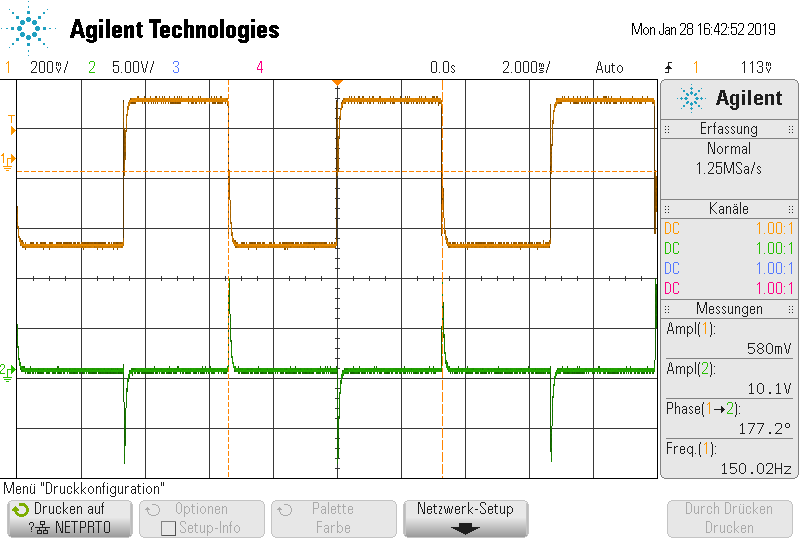
\includegraphics[width=0.8\textwidth]{Schlager/scope_20.png}
  \caption{Das Oszilloskopbild des Umkehr-Differentiators bei angelegter Rechteckspannung.}
  \label{fig:diff_recht}
\end{figure}
\begin{figure}
  \centering
  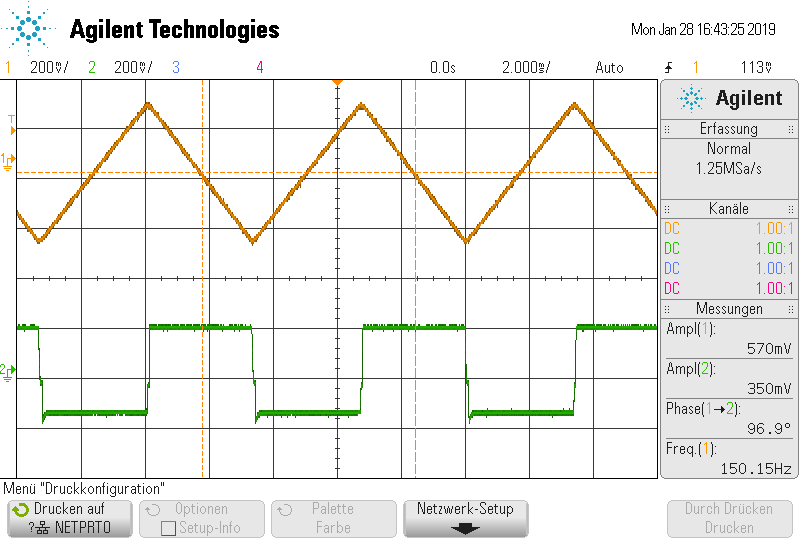
\includegraphics[width=0.8\textwidth]{Schlager/scope_21.png}
  \caption{Das Oszilloskopbild des Umkehr-Differentiators bei angelegter Dreiecksspannung.}
  \label{fig:diff_drei}
\end{figure}
\begin{figure}
  \centering
  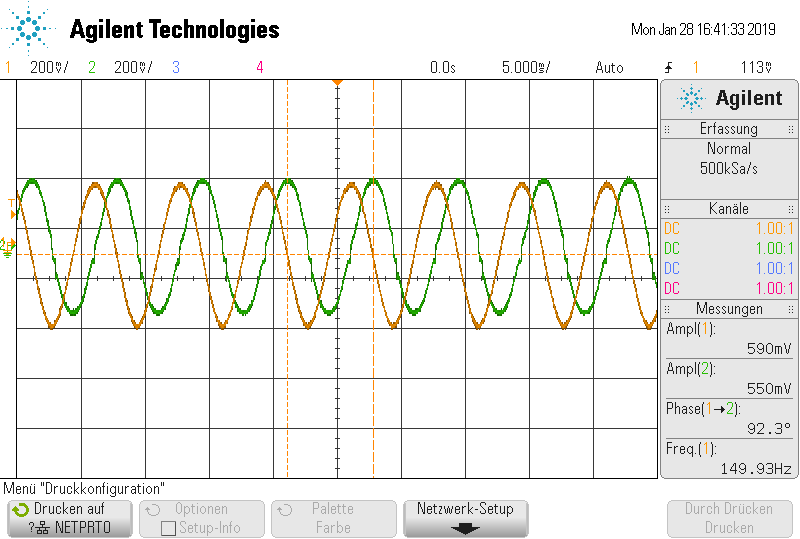
\includegraphics[width=0.8\textwidth]{Schlager/scope_19.png}
  \caption{Das Oszilloskopbild des Umkehr-Differentiators bei angelegter Sinusspannung.}
  \label{fig:diff_sin}
\end{figure}

Außerdem wird die Verstärkung $V' = U_\text{A}/U_0$ gegen die Kreisfrequenz $\omega$ aufgetragen. Dabei ist die Eingangsspannung sinusförmig. Die Messwerte sind in Tabelle \ref{tab:diff_werte} zu finden.
Die Fitfunktion nach Formel \eqref{eqn:diff_aus} lautet:
\begin{align}
  V' = k \omega.
\end{align}
Aus dem Fit, der zusammen mit den Messwerten in Abbildung \ref{fig:diff_fit} zu sehen ist, folgt:
\begin{align*}
  k = \SI{9.64(5)e-4}{\ohm\farad}.
\intertext{Die prozentuale Abweichung von dem nach Formel \eqref{eqn:diff_aus} erwarteten Wert beträgt:}
  \Delta_{k, RC} = \SI{1(5)}{\percent}.
\end{align*}

\begin{figure}
  \centering
  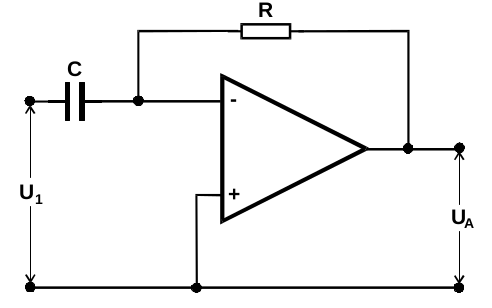
\includegraphics[width=0.8\textwidth]{build/differentiator.pdf}
  \caption{Die frequenzabhängige Verstärkung des Umkehr-Differentiators bei angelegter Sinusspannung.}
  \label{fig:diff_fit}
\end{figure}

\subsection{Schmitt-Trigger}

Die Schaltung nach Abbildung \ref{fig:schmitttrigger} liefert das Oszilloskopbild aus Abbildung \ref{fig:schmitt}.
\begin{figure}
  \centering
  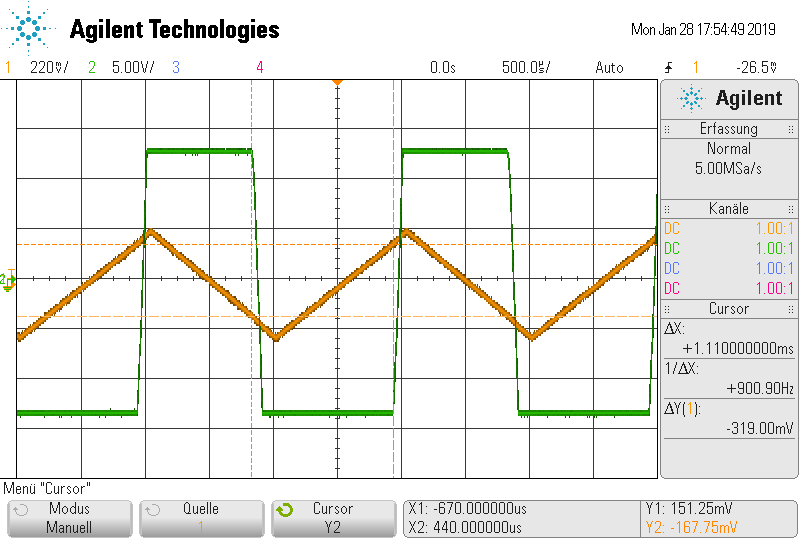
\includegraphics[width=0.8\textwidth]{Schlager/scope_22.png}
  \caption{Das Oszilloskopbild des Schmitt-Triggers mit den Spannungsmesswerten an den Stellen, an denen die Ausgangsspannung umschlägt. Hier ist die Eingangsspannung in orange und die Ausgangsspannung in grün zu sehen.}
  \label{fig:schmitt}
\end{figure}
Der Wert der eingebauten Widerstände beträgt:
\begin{align*}
  R_1 = \SI{1.002(50)}{\kilo\ohm} \quad R_\text{p} = \SI{99.7(5)}{\kilo\ohm}
  \intertext{Die Betriebsspannung beträgt:}
  U_\text{B} = \SI{14.125(50)}{\volt}.
\end{align*}
Die aus Abbildung \ref{fig:schmitt} abgelesenen Werte für die Schwellenspannung sind:
\begin{align*}
  U_\text{e, Schwelle, 1} = \SI{151(5)}{\milli\volt} \quad U_\text{e, Schwelle, 2} = \SI{-168(5)}{\milli\volt}.
\intertext{Die Abweichung von dem erwarteten Wert $R_1/R_\text{p} U_\text{B}$ betragen:}
  \Delta_{1} = \SI{7(6)}{\percent} \quad \Delta_{2} = \SI{18(7)}{\percent}.
\end{align*}

Außerdem kann in Abbildung \ref{fig:schmitt2} noch die Amplitude der Ausgangsspannung abgelesen werden. Ihr Wert und die Abweichung vom erwarteten Wert $2 U_\text{B}$ betragen:
\begin{align*}
  U_\text{A} = \SI{26.3(5)}{\volt} \quad \Delta_{U_\text{A}} = \SI{7(2)}{\percent}.
\end{align*}

\subsection{Signalgenerator}

Die Schaltung nach Abbildung \ref{fig:signalgen} liefert das Oszilloskopbild aus Abbildung \ref{fig:signalgenoszi}.
\begin{figure}
  \centering
  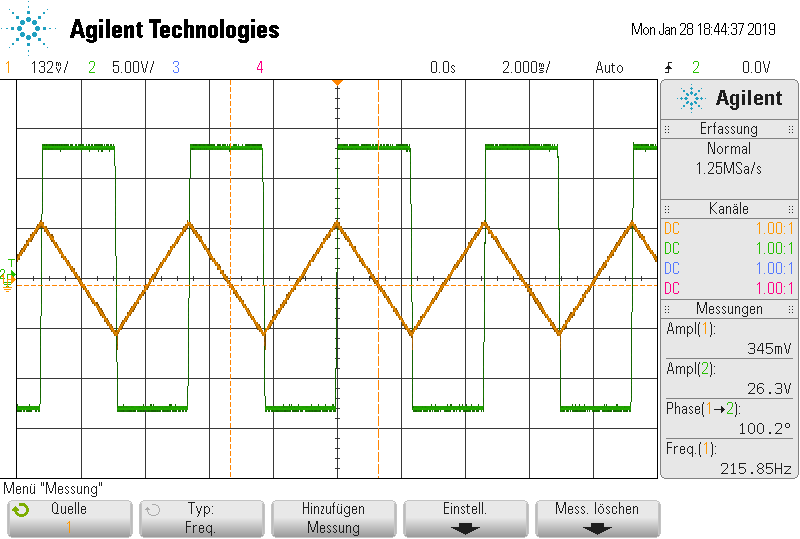
\includegraphics[width=0.8\textwidth]{Schlager/scope_25.png}
  \caption{Das Oszilloskopbild des Signalgenerators mit der generierten Dreieck- und Rechteckspannung.}
  \label{fig:signalgenoszi}
\end{figure}
Dabei haben die Bauteile folgende Werte:
\begin{align*}
  R_1 &= \SI{1.002(50)}{\kilo\ohm} \quad R_\text{p} = \SI{99.7(5)}{\kilo\ohm}\\
  R &= \SI{100.0(5)}{\kilo\ohm}\quad C = \SI{970(10)}{\nano\farad}.
\end{align*}

Die Amplituden der beiden Spannungen, sowie die Frequenz können nun mit den berechneten Werten verglichen werden.
Die gemessenen Werte sind:
\begin{align*}
  U_\text{Dreieck} = \SI{345(5)}{\milli\volt} \quad U_\text{Rechteck} = \SI{26.3(5)}{\volt} \quad \omega = \SI{1.357(6)}{\kilo\hertz}
\end{align*}
Zur Berechnung der erwarteten Dreiecksspannung wird Formel \eqref{eqn:ampl_drei} und für die Frequenz Formel \eqref{eqn:freq_signalgen} genutzt. Der erwartete Wert der Rechteckspannung beträgt erneut $2 U_\text{B}$.
Die erwarteten Werte sind also:
\begin{align*}
  U_\text{Dreieck, erw.} &= \SI{284(14)}{\milli\volt} \quad U_\text{Rechteck, erw.} = \SI{28.25(10)}{\volt} \quad \omega_\text{erw.} = \SI{3.22(17)}{\kilo\hertz}
\intertext{Die Abweichung beträgt dann:}
 \Delta_\text{$U_\text{Dreieck}$} &= \SI{22(6)}{\percent} \quad \Delta_\text{$U_\text{Rechteck}$} = \SI{7(2)}{\percent} \quad \Delta_{\omega} = \SI{58(2)}{\percent}.
\end{align*}

\subsection{Entdämpfte Schwingung}

\begin{figure}
  \centering
  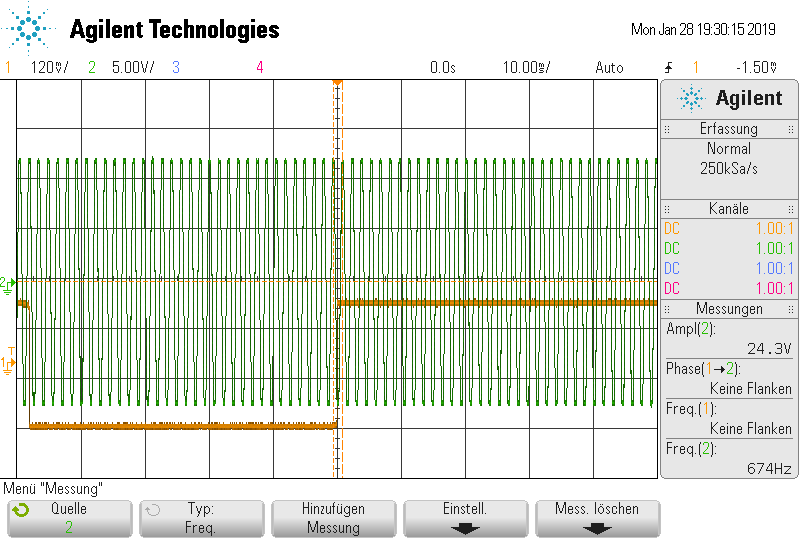
\includegraphics[width=0.8\textwidth]{Schlager/scope_28.png}
  \caption{Das Oszilloskopbild der entdämpften Schwingung.}
  \label{fig:entdaempft}
\end{figure}
In Abbildung \ref{fig:entdaempft} ist das Oszilloskopbild der entdämpften Schwingung zu sehen.
Für den Widerstand $R$ und den Kondensator $C$ werden folgende Werte gemessen. Da zwei leicht verschiedene Kondensatoren benutzt werden (siehe Messwerte im Anhang), wird für den Wert $C$ der Mittelwert aus beiden angenommen:
\begin{align*}
  R = \SI{9.96(5)}{\kilo\ohm} \quad C = \SI{22(1)}{\nano\farad}.
\end{align*}
Die gemessene Frequenz beträgt:
\begin{align*}
  \nu_\text{gem.} = \SI{674(5)}{\hertz}.
\intertext{Nach Formel \eqref{eqn:???} ist die erwartete Frequenz:}
  \nu_\text{erw.} = \SI{740(40)}{\hertz}.
\intertext{Die Abweichung beträgt:}
  \Delta_\nu = \SI{8(5)}{\percent}.
\end{align*}

\subsection{Gedämpfte Schwingung}

\begin{figure}
  \centering
  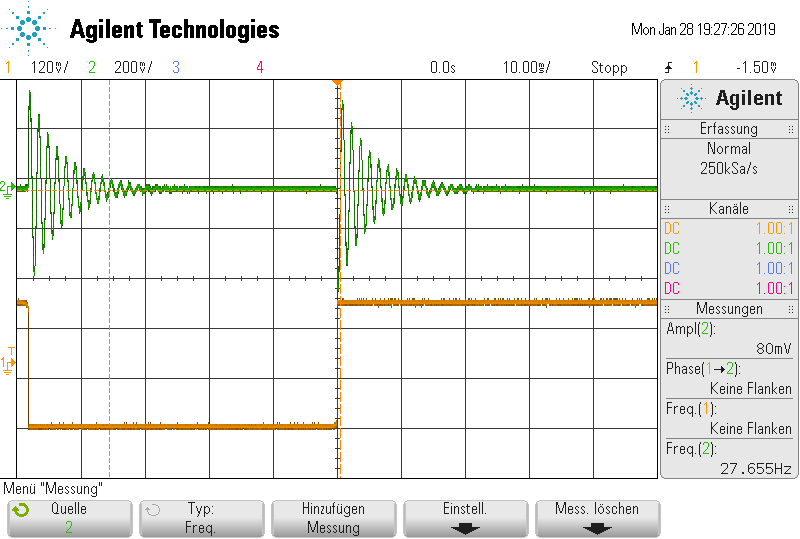
\includegraphics[width=0.8\textwidth]{Schlager/scope_26.png}
  \caption{Das Oszilloskopbild der gedämpften Schwingung.}
  \label{fig:gedaempft}
\end{figure}
In Abbildung \ref{fig:gedaempft} ist das Oszilloskopbild der gedämpften Schwingung zu sehen.
Die Werte für den Widerstand $R$ und den Kondensator $C$ sind dieselben wie im Kapitel zuvor.
An die Werte einer abschwingenden Schwingung wird nun folgende Formel gefittet:
\begin{align}
  U_\text{A} = U_0 \text{e}^{k t}.
\end{align}
In Abbildung \ref{fig:gedaempft_fit} sind die Messwerte sowie der Fit zu sehen.
\begin{figure}
  \centering
  \includegraphics[width=0.8\textwidth]{build/gedaempft.pdf}
  \caption{Die Messwerte der gedämpften Schwingung sowie der Fit an die Maxima der Schwingung.}
  \label{fig:gedaempft_fit}
\end{figure}
Die Werte aus dem Fit sind:
\begin{align*}
  k &= \SI{-209(3)}{\per\second} \quad U_0 = \SI{1.7(2)e-5}{\volt}
% \intertext{Der für $k$ erwartete Wert nach Formel \eqref{eqn:???} sowie die Abweichung des gemessenen davon betragen:}
%   20 R C &= \SI{4.4(3)e-3}{\ohm\farad} \quad \Delta_{k} = \SI{9(8)}{\percent}.
\end{align*}
Außerdem wird die Abklingzeit $\tau$ bestimmt. Sie beträgt:
\begin{align*}
  \tau = \SI{4.7}{\milli\second}
  \intertext{Der für $\tau$ erwartete Wert nach Formel \eqref{eqn:???} sowie die Abweichung des gemessenen davon betragen:}
  20 R C &= \SI{4.4(3)}{\milli\second} \quad \Delta_{\tau} = \SI{8(7)}{\percent}.
\end{align*}





% \begin{figure}
%   \centering
%   \includegraphics{build/plotElement.pdf}
%   \caption{Plot.}
%   \label{fig:plot}
% \end{figure}
%
% Tabelle für copy and paste:
% \begin{table}[h]
%   \centering
%   \begin{tabular}{S S}
%     \toprule
%     {$k$} & {$U\:/\:\si{\milli\volt}$}\\
%     \midrule
%     1 & 637.2\\
%     3 & 212.4\\
%     5 & 127.4\\
%     7 & 91.03\\
%     9 & 70.8\\
%     \bottomrule
%   \end{tabular}
%   \caption{Amplituden Rechteckspannung.}
%   \label{tab:rechtampl}
% \end{table}
